\documentclass[conference]{IEEEtran}
\usepackage[pdftex]{graphicx}
\usepackage[cmex10]{amsmath}
\interdisplaylinepenalty=2500
\usepackage{algorithmic}
\usepackage{array}
\usepackage{mdwmath}
\usepackage{mdwtab}
\usepackage{eqparbox}
\usepackage[font=footnotesize]{subfig}
\usepackage{fixltx2e}
\usepackage{url}
\hyphenation{op-tical net-works semi-conduc-tor}

% additional packages and utility commands
\usepackage{color}
\newcommand{\TODO}{\textbf{\color{red}TODO}}

\usepackage{minted}

\begin{document}

% to avoid syntax error highlighting - e.g. foo's not js ;-)
\expandafter\def\csname PY@tok@err\endcsname{}

\title{Lowering the Impact of Intrusion Detection\\
on Resources in Wireless Sensor Networks\\
using Code Generation Techniques}

\author{\IEEEauthorblockN{Christophe Van Ginneken, Jef Maerien, Christophe
Huygens, Danny Hughes, Wouter Joosen}%
\IEEEauthorblockA{iMinds - DistriNet - KULeuven\\
B-3001, Leuven, Belgium\\
Christophe.VanGinneken@student.kuleuven.be,\{firstname.lastname\}@cs.kuleuven.be}}

\maketitle

\begin{abstract}
  
Introducing intrusion detection in wireless sensor networks proofs to be a
battle for resources. Implementing and optimizing a collection of detection
algorithms to match the available resources without augmenting the production
costs beyond proportion, might very well be an unacceptable economic burden.
This paper introduces a domain specific language to formally describe such
algorithms and proposes the use of code generation techniques to automate the
production of detection software. This automated process allows for the
optimization of resource usage, more specifically the optimization of the
execution of algorithms and the use of the energy-costly wireless radio. A
prototype code generator was constructed to show that these techniques can be
implemented effectively, resulting in a combination of different intrusion
detection algorithms with less impact on the resources than the sum of the
impact of each algorithm by itself.

\end{abstract}

\section{Introduction}

Wireless sensor networks (WSN) are constructed using large numbers of
autonomous embedded devices, called nodes or motes, referring to their
dust-like properties. Their autonomy is rather absolute, being most of the time
battery-powered and deployed in open terrain. Examples of WSN include
monitoring systems in volcanic regions or flood areas. Preliminary successes
have now even steered researchers towards the introduction of WSN in cities and
homes, thus creating smart cities \cite{schaffers2011smart} and smart homes
\cite{chan2008review}.

Due to their involvement in more and more personal applications, securing these
nodes should be a priority. When we entrust these autonomous systems with some
of our most intimate information, for exameple regarding our health
\cite{stankovic2005wireless}, we would of course like them to be well suited to
protect this information.

Securing WSN, and especially single nodes, is a daunting task
\cite{perrig2004security}. Mostly due to their autonomous nature, nodes are
most of the time physically accessible. With physical access comes a wide range
of physical attacks \cite{becher2006tampering} that are hard to detect, let
alone prevent. Even if the nodes aren't physically accessible, their ways of
communicating with the outside world through various forms of wireless
communication, offer a plethora of possibilities \cite{padmavathi2009survey} to
attack them, ranging from low-level meddling with the routing of packets in the
network, up to the application level.

Securing nodes against intrusions should be a primary objective. But often this
turns out to be impossible and intrusions are sometimes only noticed
post-mortem. When prevention is not guaranteed, a second line of defence
consists in the detection of intrusions, allowing reactive systems to be
introduced to prevent future problematic situations. These intrusion detection
systems (IDS) are well-known in classic networked environments, but are not
easily transferred to the WSN world
\cite{zhang2000intrusion,djenouri2005survey}, mostly due to the wireless and
ad-hoc nature of the networks and the lack of a central point where
communication can be monitored.

But WSN bring even another problem to the table: resources. Due to their vast
deployed numbers and policy to be replaced rather than salvaged, nodes
typically need to be cheap. Their limited functional requirements allow for
them to be built using simple components without redundancy or excess margins.
This introduces an inherent problem for IDS. These systems not only typically
require a lot of resources to store detection information and have to execute
their algorithms over and an over again, but also want to inspect every single
network packets that's passing by. This way they not only would like the node
to be powered-on all the time, they also need constant access to the wireless
radio, which turns out to be the number one energy-consumer of a node.
Introducing IDS in WSN turns out to be a battle for resources.

Finally, besides the technical resources, there is also an economic resource
that plays an important part here. Given the same limited functionality, adding
a complex piece like IDS, might very well augment the production cost well
above acceptable levels. The fact that IDS algorithms are currently in a mere
state of research, would currently require a developer to read through many
research papers, making a selection of algorithms and implement them from
scratch. Even if implementations for each of these algorithms would be
available, the chance that they are applicable to the target platform is
another big if. Integrating these algorithms in itself is already a complex
matter.

Our contribution to IDS in WSN is the introduction of a domain specific
language (DSL) to formally describe IDS algorithms. The DSL is node-oriented
with a strong focus on inter-node communication and aims to allow for the
optimisation of execution of multiple IDS algorithms, thus lowering the
sequential and iterative execution of algorithms and optimizing the use of the
wireless radio.

By introducing such a formal, platform-independent language to express IDS
algorithms and accompanying this language with a code generation framework,
offers an end-to-end solution to many of the problems introduced above:
research output would be directly applicable in a development environment. The
code generation framework allows developers to simply select algorithms and
have platform-specific code without any effort. Due to the possibility to
optimize the use of resources, the impact of introducing IDS on resources in
WSN can be lowered to such extend that more algorithms can be added, thus
augmenting the barriers for intruders, which can help to reduce the number of
successful intrusions.

The remainder of this paper proceeds as follows: section \ref{section:related}
introduces the field of IDS in WSN by means of several IDS algorithms from
research papers. Section \ref{section:problem} describes the problem space in
detail, covering the different parties involved and their contributions.
Section \ref{section:solution} introduces our proposed overall solution, which
is further detailed in sections \ref{section:foo-lang} and
\ref{section:prototype}, which respectively present our domain specific
language, FOO-lang, focusing on the optimization of the organization of
functionality, as well as a prototype implementation of a code generator
framework to complement the language. Section \ref{section:evaluation}
evaluates the prototype implementation and determines if the theoretical merits
of introducing FOO-lang, are actually viable. Finally, section
\ref{section:conclusions} presents our conclusions and proposes topics for
future research to fine-tune the initial findings.

\section{Related Work}
\label{section:related}

Securing any network initially tries to prevent intrusions from happening. This
should of course be a primary concern. But not all intrusions can be prevented
and we need to fall back to detecting intrusions. In this section we take a
look at recent contributions in this field.

Intrusion, or attacks, on computer networks can take many forms. In the case of
WSN this classification needs to be extended even further. In
\cite{padmavathi2009survey} a good overview of both is presented, showing
clearly that WSN suffer from their wireless-communication and broadcast nature.
This causes many attacks based on e.g. eavesdropping to be nearly impossible to
detect while they are happening. Only when the actual intrusions, based on
collected information, have happened, the intrusion could possibly be detected
given the after-effects. This means that we can't cover the entire spectrum and
need to focus on what is feasible.

Research into IDS in WSN typically focuses around two major topics that
complement the architecture of WSN: the nodes as single entities and the
network as a group of such nodes. Both are important because the group cannot
decide without members that detect malicious behavior and a group-based
decision is often needed because nodes can easily miss out on certain events
that could indicate intrusions, due to their wireless and not-always-on nature.

\subsection{Detecting Intrusions}
\label{subsection:detecting}

There are many different ways to construct a taxonomy for intrusion detection,
but common themes do show. According to \cite{mishra2004intrusion} and
\cite{ioannis2007towards} there are three major categories: anomaly detection,
signature or misuse detection, and specification-based detection. In
\cite{alrajeh2013intrusion} the authors agree mostly with this topology, but
add the notion of hybrid intrusion detection systems and cross layer intrusion
detection systems as recent advances in research. Although these additional
categories offer very interesting prospects, the authors have to admit that the
impact on the resource-constrained sensor nodes might still be too high.

The meshed network topology of WSN and its routing protocols has produced many
related attacks and each of these attacks has been the focus of many research
papers presenting algorithms to detect them. In the following paragraphs we
take a look at some of the popular ones.

In a wormhole attack, an artificial low-latency link is created between two
distant nodes in the network. This causes the routing protocol to divert more
traffic through this link, offering the attacker with an abundance of packets
to inspect. In \cite{maheshwari2007detecting} an algorithm is proposed to allow
nodes to determine if a wormhole is actively present. In essence, the algorithm
resides on the exchange of neighbour lists to allow nodes to determine if
unexpected substructures are present in the graph representing the network.

The wormhole attack typically doesn't need to alter any nodes and can make do
with adding two additional nodes in the network. When this addition goes
unnoticed, the wormhole can successfully be constructed. Another attack that is
related to the wormhole is the sinkhole. When launching a sinkhole attack, as
described in \cite{krontiris2008launching}, the attacker first needs to
compromise an existing node. He can achieve this without changing the node's
software and thus control the node in an external way, e.g. using a laptop.
Being in control of the node, the attacker will alter the information provided
to the distributed routing algorithm to make his captured node look
\emph{attractive} to the surrounding nodes and thus draw as much traffic as
possible to itself. The sinkhole attack is typically a foundation for other
routing level attacks, such as selective forwarding, modification of packets or
even dropping them altogether. In its simplest form, the sinkhole offers the
attacker with lots of packets to analyse and use to gather information about
the network and its functionality. Detecting sinkholes is very hard and often
is only possible based on other attacks that are supported by the sinkhole.
When the sinkhole is used to implement selective forwarding,
\cite{ngai2006intruder} proposes an algorithm that allows a base station, the
aggregating master node where all nodes typically send their information to, to
observe missing data from nodes in the same area in a statistical way.

More typical attacks such as flooding, the sybil attack, rushing,\dots are
presented in \cite{wood2002denial} and \cite{djenouri2005survey}.

\subsection{Cooperative Decision Making}
\label{subsection:coorperative}

As in many other situations, a group is often stronger that the sum of its
individual components. This is surely the case for WSN. Because not all nodes
are always actively participating in the network, some nodes might miss queues
that would otherwise lead them to detect intrusions. It is hardly impossible
for a single node to detect a complex attack by itself. Therefore a second
important research topic consists of cooperative algorithms used to combine
information from single nodes into a group-based decision about alleged
intrusions and intruders.

In \cite{krontiris2009cooperative}, the authors first present a theoretical
foundation the analyse cooperative algorithms. Given these foundations they
continue to present an algorithms consisting of 5 phases. It essentially
implements a voting system to identify an intruder based on the Guy Fawkes
protocol \cite{anderson1998new} to exchange suspected intruder information and
allow distributed authentication of those so called votes. Based on these
authenticated votes, a distributed decision can be made about the commonly
identified intruder.

A distributed, cooperative algorithm can sometimes be implemented locally. This
is illustrated by the reputation-based detection algorithm introduced in
\cite{ganeriwal2008reputation}. Using this algorithm, nodes can exchange
information about the reputation of other nodes. Combining this information
allows them to decide about their trust in a given node, using more than only
their own observations.

\subsection{Software Attestation}
\label{subsection:attestation}

A research topic that lives parallel to the detection/cooperation duality is
that of software attestation. Software attestation basically tries to offer
algorithms for exchanging information about the software that is running on a
node, and aims to identify nodes that can no longer prove that their content is
unaltered. Examples of evolving algorithms to implement this functionality
include SWATT \cite{seshadri2004swatt}, ICE/SCUBA \cite{seshadri2006scuba} and
SAKE \cite{seshadri2008sake}. The list of authors shows that this topic lives
strong in certain groups.

Software attestation is hard and many details can cause an algorithm to fail.
Interesting is the discussion surrounding this topic that was started by
\cite{castelluccia2009difficulty}, in response to the previously mentioned
papers. In \cite{perrig2010refutation} the authors of the original papers
counter many of the objections made to their work, but the general feeling is
that even in the best conditions, there is always a backdoor that allows to
circumvent even the most ingenious algorithm to perform software attestation.

\section{Problem Analysis}
\label{section:problem}

The problem of introducing IDS in WSN is much broader than simply the
implementation of a software component. It starts at the very foundations of
WSN. In contrast with for example SNORT \cite{roesch1999snort}, there is
currently no community based collection of algorithms that can be implemented.
The reason is mostly due to the lack of a central/external location where all
network traffic can be analyzed out-of-band. In WSN it's not possible to create
a single entity that will monitor the WSN as is the case in a classic wired
network. Therefore, all algorithms typically evolve independently, without any
cohesion.

Even more, all of these algorithms lack a common, formal notation. In the case
of SNORT, a detection language is provided and new signatures are added on a
regular basis, creating an ever growing rule base, capable of detecting even
the newest of attacks out there.

If implementers of WSN want to add IDS to their network, and therefore to the
nodes in the network, they are facing no small task: first they need to collect
research papers, from which they need to extract the proposed algorithms. Even
if the papers would come with an implementation of their algorithm, the chance
that the implementation matches the target platform of the newly created WSN is
slim.

Simply implementing the different algorithms in sequence, or reusing existing
implementations if they would be available, is also no valid option. All of
these algorithms typically perform the same actions: first they analyze each
incoming packet and collect information about nodes, and secondly at given
intervals, they loop over all known nodes, checking the aggregated information
about them and make decisions about the trust to put in them. While performing
all of these tasks, the algorithms typically also exchange information with
other nodes to complement their own findings.

If such algorithms would be simply combined in a sequential way, the resulting
code would be far from optimal and would consume many of the resources of the
node it runs on: the repetitive parsing of the received packets would result in
much longer processing times than needed, while the chattiness of the
inter-node communication would result the wireless radio being on much more
than wanted.

The cost to implement multiple algorithms over and over again, because due to
the need to optimize the code organisation, would soon outweigh the available
budget of any WSN implementation. If not, the risk to make mistakes in the
sometimes complex algorithms or the lack of flexibility to change sets of
detection algorithms on a regular basis, or simply add a new algorithm in an
easy way, are all very valid reasons to not go down this way. But we still need
to be able to add some form of IDS to WSN.

\section{Proposed Solution}
\label{section:solution}

Different approaches are possible to address the problems identified above. A
major contribution would consist in the creation of a software framework that
accommodated some of the typical usage patterns: a generic payload parser could
be envisaged that allows algorithms to hook in using callbacks, thus making
sure that the parsing is only done once and not repeated for each algorithm.
Secondly, such a framework could collect all outgoing messages and combine them
in a single outgoing packet at the end of a cycle of the node's event loop.

Such a framework comes with guidelines on how to use it, but still relies on
the good behaviour of its users. Also, the integration of the algorithms with
this framework would still be manual work and reconfiguration would typically
impact this part of the implementation. Finally, such a framework does support
the implementation, but still requires thorough analysis of research material
and extraction of the relevant algorithms.

In the case of SNORT \cite{roesch1999snort}, or any other classic network IDS
for that matter, the central detection engine accepts formal descriptions of
signatures of attack patterns. Because it isn't possible to create such a
central component once, there has been no urge to describe detection algorithms
in a formal way. If we now introduce code generation techniques to convert a
formal, platform-independent description of detection algorithms, and generate
this central component, we can bridge the remaining gap.

Code generation allows for the creation of code that implements the actual
algorithm. The algorithm can be described in a platform-independent way,
therefore allowing reuse of the algorithm on multiple platforms. The generated
code can further access a minimal software framework that covers common tasks
and/or platform specific functionality.

Given formal descriptions of the algorithms, a implementer of a new WSN
application could simple select a set of algorithms, feed their formal
description to the code generator and automatically receive platform-specific
code, optimized for execution and communication.

A formal description of detection algorithms would not only be beneficiary to
implementers. Also to researchers such medium would offer substantial benefits.
Formal descriptions of these algorithms not only allows for generation of code,
but the same descriptions can be loaded into simulators and be investigated in
combination with other algorithms \cite{mernik2005and}, formal analysis of the
algorithms would be an interesting option. Further, describing the algorithms
in a platform-independent way, would increase their usefulness and allow for
more complex algorithms to be abstracted.

\section{Introducing FOO-lang}
\label{section:foo-lang}

The central component of our proposed solution is a formal description of
intrusion detection algorithms. This formal description can be realized using a
domain specific language (DSL). Before actually defining a new language, it is
important to ensure that the reasons to do so are legit. Too often languages are
implemented too quickly, where coding conventions or frameworks with well
thought-out API's fit the bill quiet nicely.

The line can not be drawn in a black and white fashion and DSL do have
benefits, but don't come for free \cite{mernik2005and}. Many good reasons why
to implement a DSL, or not, can be found in \cite{van2000domain},
\cite{mernik2005and} and \cite{fowler2010domain}. Based on these, we try to
justify our choice to propose a DSL for this solution.

\subsection{Justification of the Use of a DSL}
\label{subsection:justification}

The primary goal is the proposed solution is to avoid the creation of bad code
that drains the limited resources of a node. Two basic examples are presented
to illustrate this bad behaviour: repetitive execution of the same tasks, such
as parsing or iterating over a set of known nodes and the use of the wireless
radio.

The latter can be covered by a framework, as illustrate earlier. It comes with
an obligation to actually use the framework. One cannot protect users against
their own stupidity if they don't follow the rules. The former is a bit
trickier. Let's say that we would use the C language as a lingua franca to
complement the framework, which hides the platform specific parts. This would
be valid, but offering a complete language would soon result in loops that
break with the guidelines and would undermine the conceptual idea of optimizing
the organisation of the functionality.

Restricting the formal description to a subset that doesn't allow for
constructions that violate the goals, is in this case a valid reason to tend
towards a DSL. Introducing a DSL further also allows for more functional ways
of handling the concepts that are part of the domain. In this case the domain
clearly consists of inter-operation between nodes and local processing of
algorithms that typically deal with sets of nodes. Although that C comes close
to a lingua franca amongst both researchers and implementers, it is still a
very low-level language with very little support for concise operations such as
pattern matching, event-driven-ness,\dots.

If C doesn't fit this profile, maybe another language does. During the early
days of our research, we looked at a language that seems to fit the required
functionality like a glove: Erlang \cite{armstrong1993concurrent}. It comes
with strong communication paradigms, has pattern matching, is concurrent and
event-driven by nature,\dots and according to \cite{wong1998compiling} it even
can be translated to C. This road looked very promising, but as with any other
general purpose language, it was to capable and would allow for constructions
that would thwart the envisaged optimizations.

Our final conclusion is that a real domain-functionality inspired DSL, that
permits analysts to express the detection algorithms without overhead and
without risk of introducing ill behaviour, is the way to go forward.

\subsection{Design Principles for FOO-lang}
\label{subsection:design}

Designing a language is an exciting task, but at the same time comes with great
responsibility. It is important to make the language ``as simple as possible,
but not simpler'' - to paraphrase Albert Einstein. The language should come
with enough support to write concise code, but not become obfuscated. The
constructs it offers should be applicable in generic combinations with each
other and be especially transparent in use.

On the other hand, in this case, it is important that the language also
restricts the user without limiting his expressiveness or making certain
expressions unintuitive.

Starting from this last requirement, one of the most important things that
should not be available is \emph{loops}. If we want to control the way lists of
data are handled, we need control over the loops over that data. In case of
this specific domain, data is centralized around \emph{nodes}, so loops are
typically targeting nodes. To meet this restriction and still offer the analyst
a way to functionally handle nodes, scheduling and events are introduced. In
stead of explicitly constructing a loop, functionality can be scheduled or
attached to certain events that happen on the collection of nodes. This way,
the intended loop is actually abstracted to its functional meaning and can be
nicely handled and combined with other execution strategies.

This is actually the core of the language and this is also where it derived its
name from: Function Organization Optimization.

A second important feature of the language is be that it should feel natural.
Luckily, in the case of embedded systems and WSN in specific, both researchers
and implementers share a common language. Most development on these systems is
done in C, and both parties know this language well. The choice to mimic C for
a lot of the general syntax is therefore an open door.

FOO-lang also borrows basic syntax from object-oriented (OO) languages, in that
respect that it bears the concept of methods that can be called upon
\emph{objects}. The language doesn't provide any means to define or instantiate
objects. The \emph{nodes} domain controls the availability of these objects,
creating them and providing them to the functions that are defined.

To avoid typical constructions that often also require loops, the concept of
pattern matching is introduced. Here a pattern of non-variables and variables
can be provided to functions that support them. If such a function can match
the non-variable part of the pattern, the variables in the pattern take on the
corresponding values of the data against which the match was performed. It is
obvious that this will typically be used to analyze incoming data when
communicating between nodes. Often used in conjunction with this functionality
are list literals, that allow to combine different (non-)variables.

To allow complex code to be introduced, the language also provides a way to
import external functionality. This feature is provided through an statement
that allows to define the prototype of the imported function, which can then be
used as any other function.

One final feature is important: type inference. FOO-lang tries to limit the
need for typing information. Based on declaration and usage, most types can be
inferred. In doing so, the language tries to focus on the functionality and not
on the technical implementation. This mainly targets the analysts and
researcher that now can focus on the bare essence. Also, typing can be
platform-dependent and we want the descriptions to be platform-independent.

\subsection{The Actual Language}
\label{subsection:language}

In the previous paragraphs the design principles of FOO-lang were introduced.
In this section we take a look at an actual piece of FOO-lang code and see how
these design principles are realized.

Based on the algorithms that were introduced in many of the consulted papers, a
pretty common structure for these algorithms can be found: when new data is
received, the algorithm wants to process this, at regular intervals the
algorithm wants to validate the information it has on known nodes and at all
times, the algorithm might want to communicate with other nodes to exchange
information. Given this structure, we now introduce the \emph{hello world}
example for FOO-lang: \emph{heartbeat}.

Heartbeat can be considered the most elementary intrusion detection algorithm
possible, that still contains all aspects identified with other more complex
algorithms.

\inputminted[linenos,xleftmargin=2mm,numbersep=1mm,frame=lines,framesep=2mm,fontsize=\footnotesize,fontfamily=courier]{js}
  {heartbeat.foo}
\captionof{listing}{Example implementation of \emph{heartbeat}.\label{lst:heartbeat}}

The underlying concept boils down to availability. As long as we receive
regular updates from a given node, we trust it. When it fails to produce a
heartbeat on a regular interval, we no longer trust it. The resulting FOO-lang
code is presented in listing \ref{lst:heartbeat}.

At the top of the listing we see the \emph{module} construct. It marks the
start of the definition of a group of related constructs.

Next a set of \emph{const}ants is defined. Although not mandatory, use
functional names for certain parameters of the algorithm should be considered
good practice. Here we see that the constants are not typed. They can be, but
they mustn't. Based on the value, FOO-lang will infer the type.

Although no specific order is mandatory, \emph{import}ing external
functionality is typically performed close to the start of the module. The
import states the external module where the functionality comes from. This
could be a FOO-lang module, but also any other C module with custom defined
functions. In this case we import functions to compute and compare SHA-1 hashes
and access to the current time.

The central concept of the domain are \emph{nodes}. The domain logic will keep
track of nodes and provide access to them. From a module's point of view, we
can add properties to nodes to allow the algorithm to store specific
information with each node. This is done through \emph{extend}ing the
\emph{nodes} with additional properties.

Time to define the actual functionality. This consists of three parts: handling
incoming information, validating nodes and broadcasting a heartbeat.

Handling incoming data is implemented by responding to an event targeting
nodes, more specific the \emph{receive} event. In theory, this event can be any
method that is defined on an object and as such the event-driven system can be
considered some form of aspect-oriented programming. The signature of the
function that can handle the event is the same as that of the corresponding
method that triggered the event.

Interesting to note here is the use of the entire nodes domain as a target for
the event. Not only messages received by our own node will be handled here.
Given the wireless communication medium, any node can \emph{overhear}
communication between two other nodes, given that the sender of those nodes is
within its range. These messages will also pop up here and can be valuable.

The implementation of the handling function consists of a mix of typical C
constructs and a few additions. Most notably is the \emph{case} construct that
allows to define multiple situations that might be handled. It is used to
handled different situations with the same object, here the payload of an
incoming packet. The contains method is executed on the payload and takes a
pattern to match. The pattern consists of a list literal with non-variables and
variables. The non-variable in this case is an \emph{atom}, and is prefixed
with a `\#' character. It serves as a uniquely identifiable marker and abstracts
the underlying implementation. It avoids the use of constants in this case. If
the contains function encounters the representation of the \emph{heartbeat}
atom, it will map the other variables in the pattern to the data that follows
it. Because some of the types of these

\inputminted[linenos,xleftmargin=2mm,numbersep=1mm,frame=lines,framesep=2mm,fontsize=\footnotesize,fontfamily=courier]{js}
  {reputation.foo}
\captionof{listing}{Example reputation-based decision making.\label{lst:reputation}}

variables might not be trivial to infer, it is possible to explicitly express
these types. In this specific case inference would be possible, based on the
use of the variable in the following handling code, which is almost completely
pure C.

A second function is defined, along with a scheduled execution strategy.
FOO-lang here tries to be very fluent in its syntax and therefore the second
declaration reads exactly as it is meant to be: ``at every validation interval
with (all) nodes do function ...''. Two constructs here are combined in a
typical situation: a scheduling using the \emph{@every} annotation and the
scoped execution of function with the \emph{with} construct. The parameter of
the handling function is a \emph{node} and the implementation of the function
can be read completely as pure C code.

The final function is again a scheduled execution strategy based on the
\emph{@every} annotation, but now scoped to our own node with a handler
implemented using a named function. The implementation uses the
\emph{broadcast} method on the global collection of nodes to send out its
heartbeat.

Although this example does not contain all possible constructs and combinations
of constructs, it is very representative for the typical intrusion detection
algorithm and shows in a limited scope the possibilities of FOO-lang.

Listing \ref{lst:reputation} shows the implementation of the reputation-based
decision algorithm introduced by \cite{ganeriwal2008reputation}. We will not
comment it in detail, but given the previous elementary \emph{heartbeat}
example, the extended functionality used in this example should be trivial to
understand. The most important additions are the introduction of the
\emph{don't care} operator `\_' and the use of dynamic pattern matching such as
$<$ now(). Further does this example expose methods that are defined on
lists.

\section{Prototype Code Generator}
\label{section:prototype}

Defining a language is one thing. It should of course also be possible to
generate code from it that actually solves some of the problems we identified
earlier. In the case of a language, the only real proof is in building an
actual code generator.

We have build a prototype code generator for FOO-lang using Python and ANTLR
\cite{antlr3}. The implementation tries to be as generic as possible and is
based around transformations of abstract syntax trees (AST) an a semantic model
\cite{fowler2010domain}.

The FOO-lang code is parsed using a parser generated by the ANTLR tool. This
produces an AST, which in its turn is transformed into a semantic model using a
visitor. The semantic model represents that actual meaning of the
implementation. From a project point of view, the DSL is merely a textual
representation of the semantic model and the parser and first visitor allow us
to easily populate the model.

The initial model is an exact representation of the FOO-lang code that was
parsed. This means for example that not all types are well defined. A second
visitor, now targeting the semantic model, is used to check all types and try
to infer those that are still marked \emph{unknown}.

With all types known, the model is semantically complete and we can move to the
next phase: construction of a code model. A code model can actually be
considered an AST that later on can be persisted as code again. The initial
code model that is constructed from the semantic model typically contains all
the language features available in FOO-lang. The construction is done partly by
the generic generator and partly by the \emph{nodes} domain.

The back-end of the code generator aims to be language and platform
independent. Both language and platform are exchangeable plug-ins to the
generator. With the initial code model based on the full set of language
constructs of FOO-lang, it is clear that the transformations that need to be
performed by these plug-ins are the migration of constructs that are not
literally available in the target language or platform.

The resulting code model is an AST that can be emitted in the desired language
and conforming to the target platform.

\section{Evaluation}
\label{section:evaluation}

To evaluate the prototype we have chosen to use a barebone system based on the
Atmel ATMEGA1284p micro-controller (mcu) \cite{datasheet:atmega1284p} and the
Digi XBEE S2 Zigbee module \cite{datasheet:xbee}. To drive the hardware a
minimalistic library was used.

The reason for this at first sight unusual setup is simple though: relying on
basic hardware and software allows us to validate that the generator is capable
of generating code even for the most basic environment available. Any step up,
both in hardware or software would offer better and higher abstractions that
would make it easier to generate code for that situation. It shows that the
requirements of the generator towards the platform are minimal, don't rely on
advanced frameworks or operating systems and can therefore be applied in any
environment, targeting any platform.

For the evaluation we constructed a mini WSN consisting of three nodes: an
end-device, a router and a coordinator. The end-device and the router were
completely autonomous nodes, while the coordinator consisted of an XBee module,
directly connected to a computer via a USB break-out board, allowing serial
access via a terminal.

The end-device implements the heartbeat and reputation algorithms and monitors
if the router actually forwards its messages. Next to the IDS logic a
light-sensor is being processed and its readings are forwarded to the
coordinator.

The router is also implemented using both algorithms, as to allow both the
end-node and the router to monitor each others' heartbeat. For the router
different implementations were also constructed to allow testing with a fully
cooperating router, a partially failing router and a non-cooperative router.

Two aspects were to be evaluated: functionality and resource usage. On a
functional level, the nodes performed as expected from the algorithms.
Heartbeats were correctly broadcast and monitored, reputation computations were
performed as theoretically expected.

With respect to resource usage, we analyzed the generated source code to
confirm that the generated constructions indeed were better than simple
sequential constructions. At run-time the content of the packets that were sent
showed that when possible multiple information was aggregated into a single
packet, thus reducing some of the added chattiness caused by the introduction
of the IDS algorithms.

\section{Conclusions and Future Work}
\label{section:conclusions}

WSN nodes typically respond to events in their environment or perform their
tasks at clearly scheduled intervals. Applying a language that has these
concepts at its core, allows focus on the bare essence and reuse of best
practices at the generation level. The rather limited functional domain of WSN
proofs to be a wonderful candidate for applying code generation techniques.

The ideas proposed in this paper and the prototype are very basic foundations.
They show that using code generation techniques can be used to combine
different, independent algorithms in a fully automated way, while offering
better resource usage than simply sequentially combining the algorithms.

These preliminary steps open up a broad range of possible tracks to explore. On
one hand our goal is to collect as many relevant research papers as possible
and extract the algorithms from them, implementing them using FOO-lang. This
will undoubtedly lead to extensions to the language and its core libraries. On
the code generation front itself, the generator has to be lifted from the
prototype level up to production quality. Next, many optimizations can be added
to it: functional code inlining, continuation-passing style code
structuring,\dots

But on a higher level other challenges are also prominently present: having
formal, platform-independent descriptions of algorithms, allows for simulation
and thorough analysis of their behaviour, both by themselves as in
combinations. Finding ways to combine as many algorithms as possible in a
single generated solution will enable implementers of WSN to add a decent level
of intrusion detection to their solutions with almost a single click.

Finally we hope that this paper might be received as a call-for-participation
by all IDS in WSN researchers and will lead to an ever growing collection of
formal descriptions available to those that need them.

\section*{Acknowledgements}
\label{section:acknowledgements}

We would like to thank the reviewers for their thoughtful and helpful comments
that enhanced the readability of this paper. Our gratitude and respect also
goes out to all members of the WSN work group at KU Leuven for creating the
nurturing environment where these ideas could grow.

\bibliographystyle{IEEEtran}
\bibliography{referenties}

\end{document}

% \begin{figure}[!t]
% \centering
% 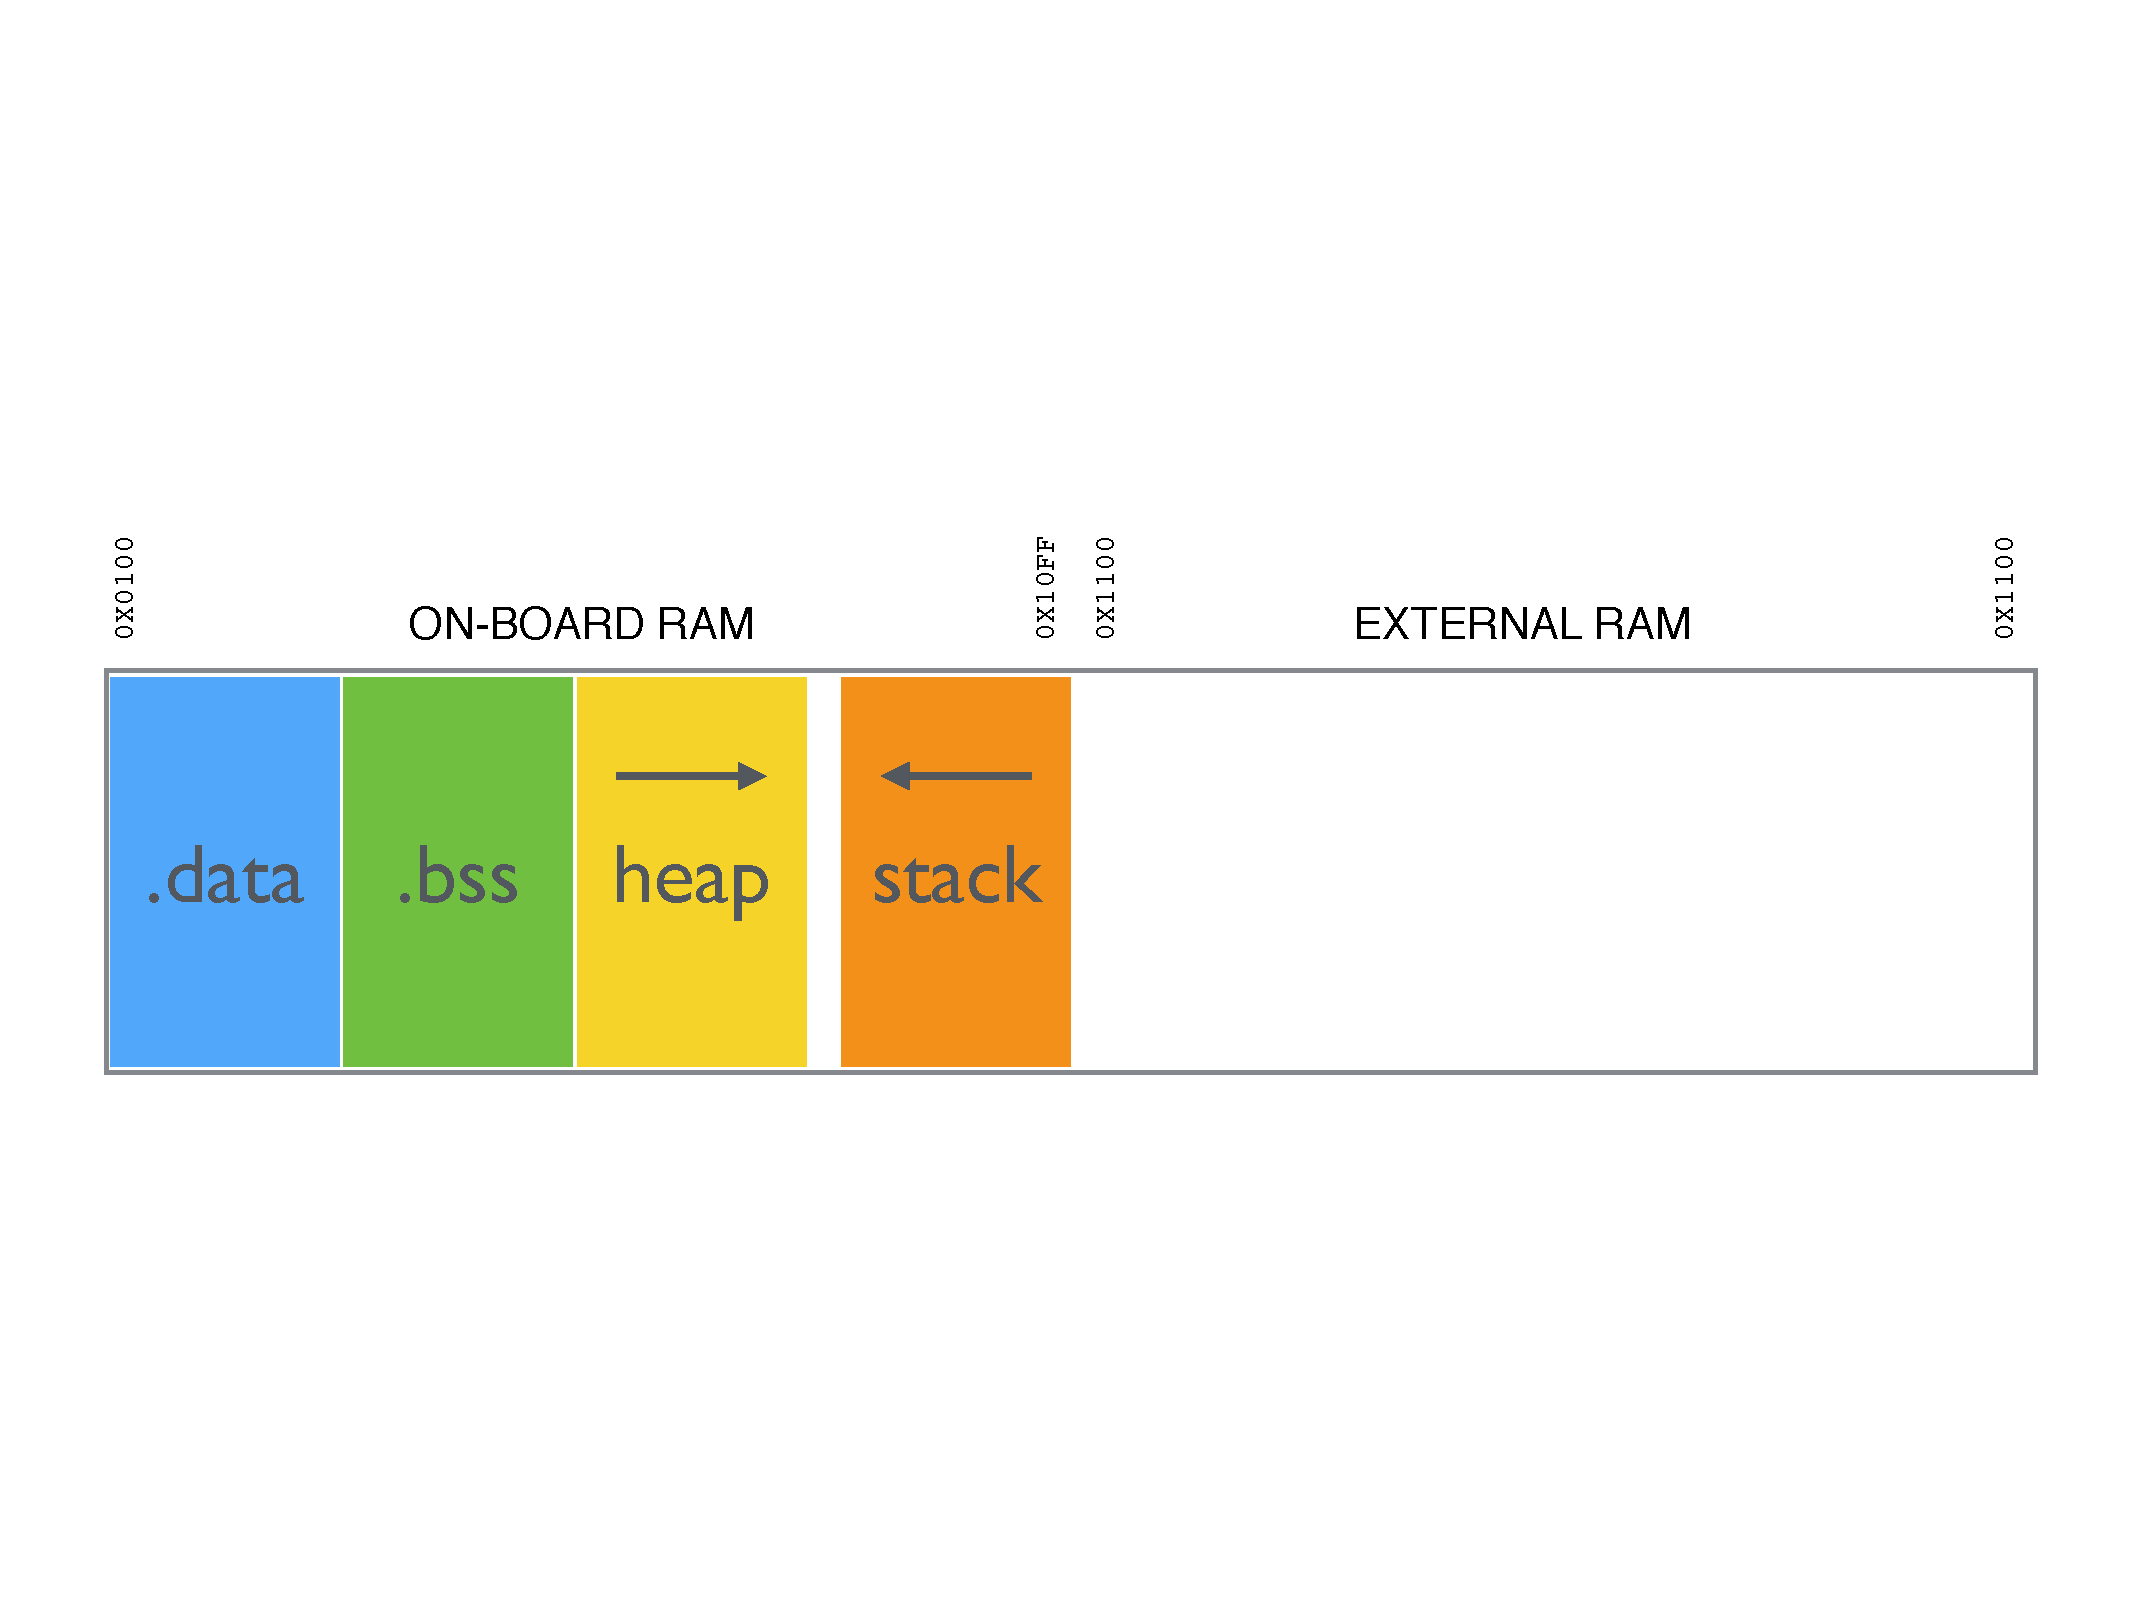
\includegraphics[width=2.5in]{resources/avr-ram-map.pdf}
% \caption{Simulation Results}
% \label{fig_sim1}
% \end{figure}
% 
% \begin{figure*}[H]
% \centering
% \subfloat[]{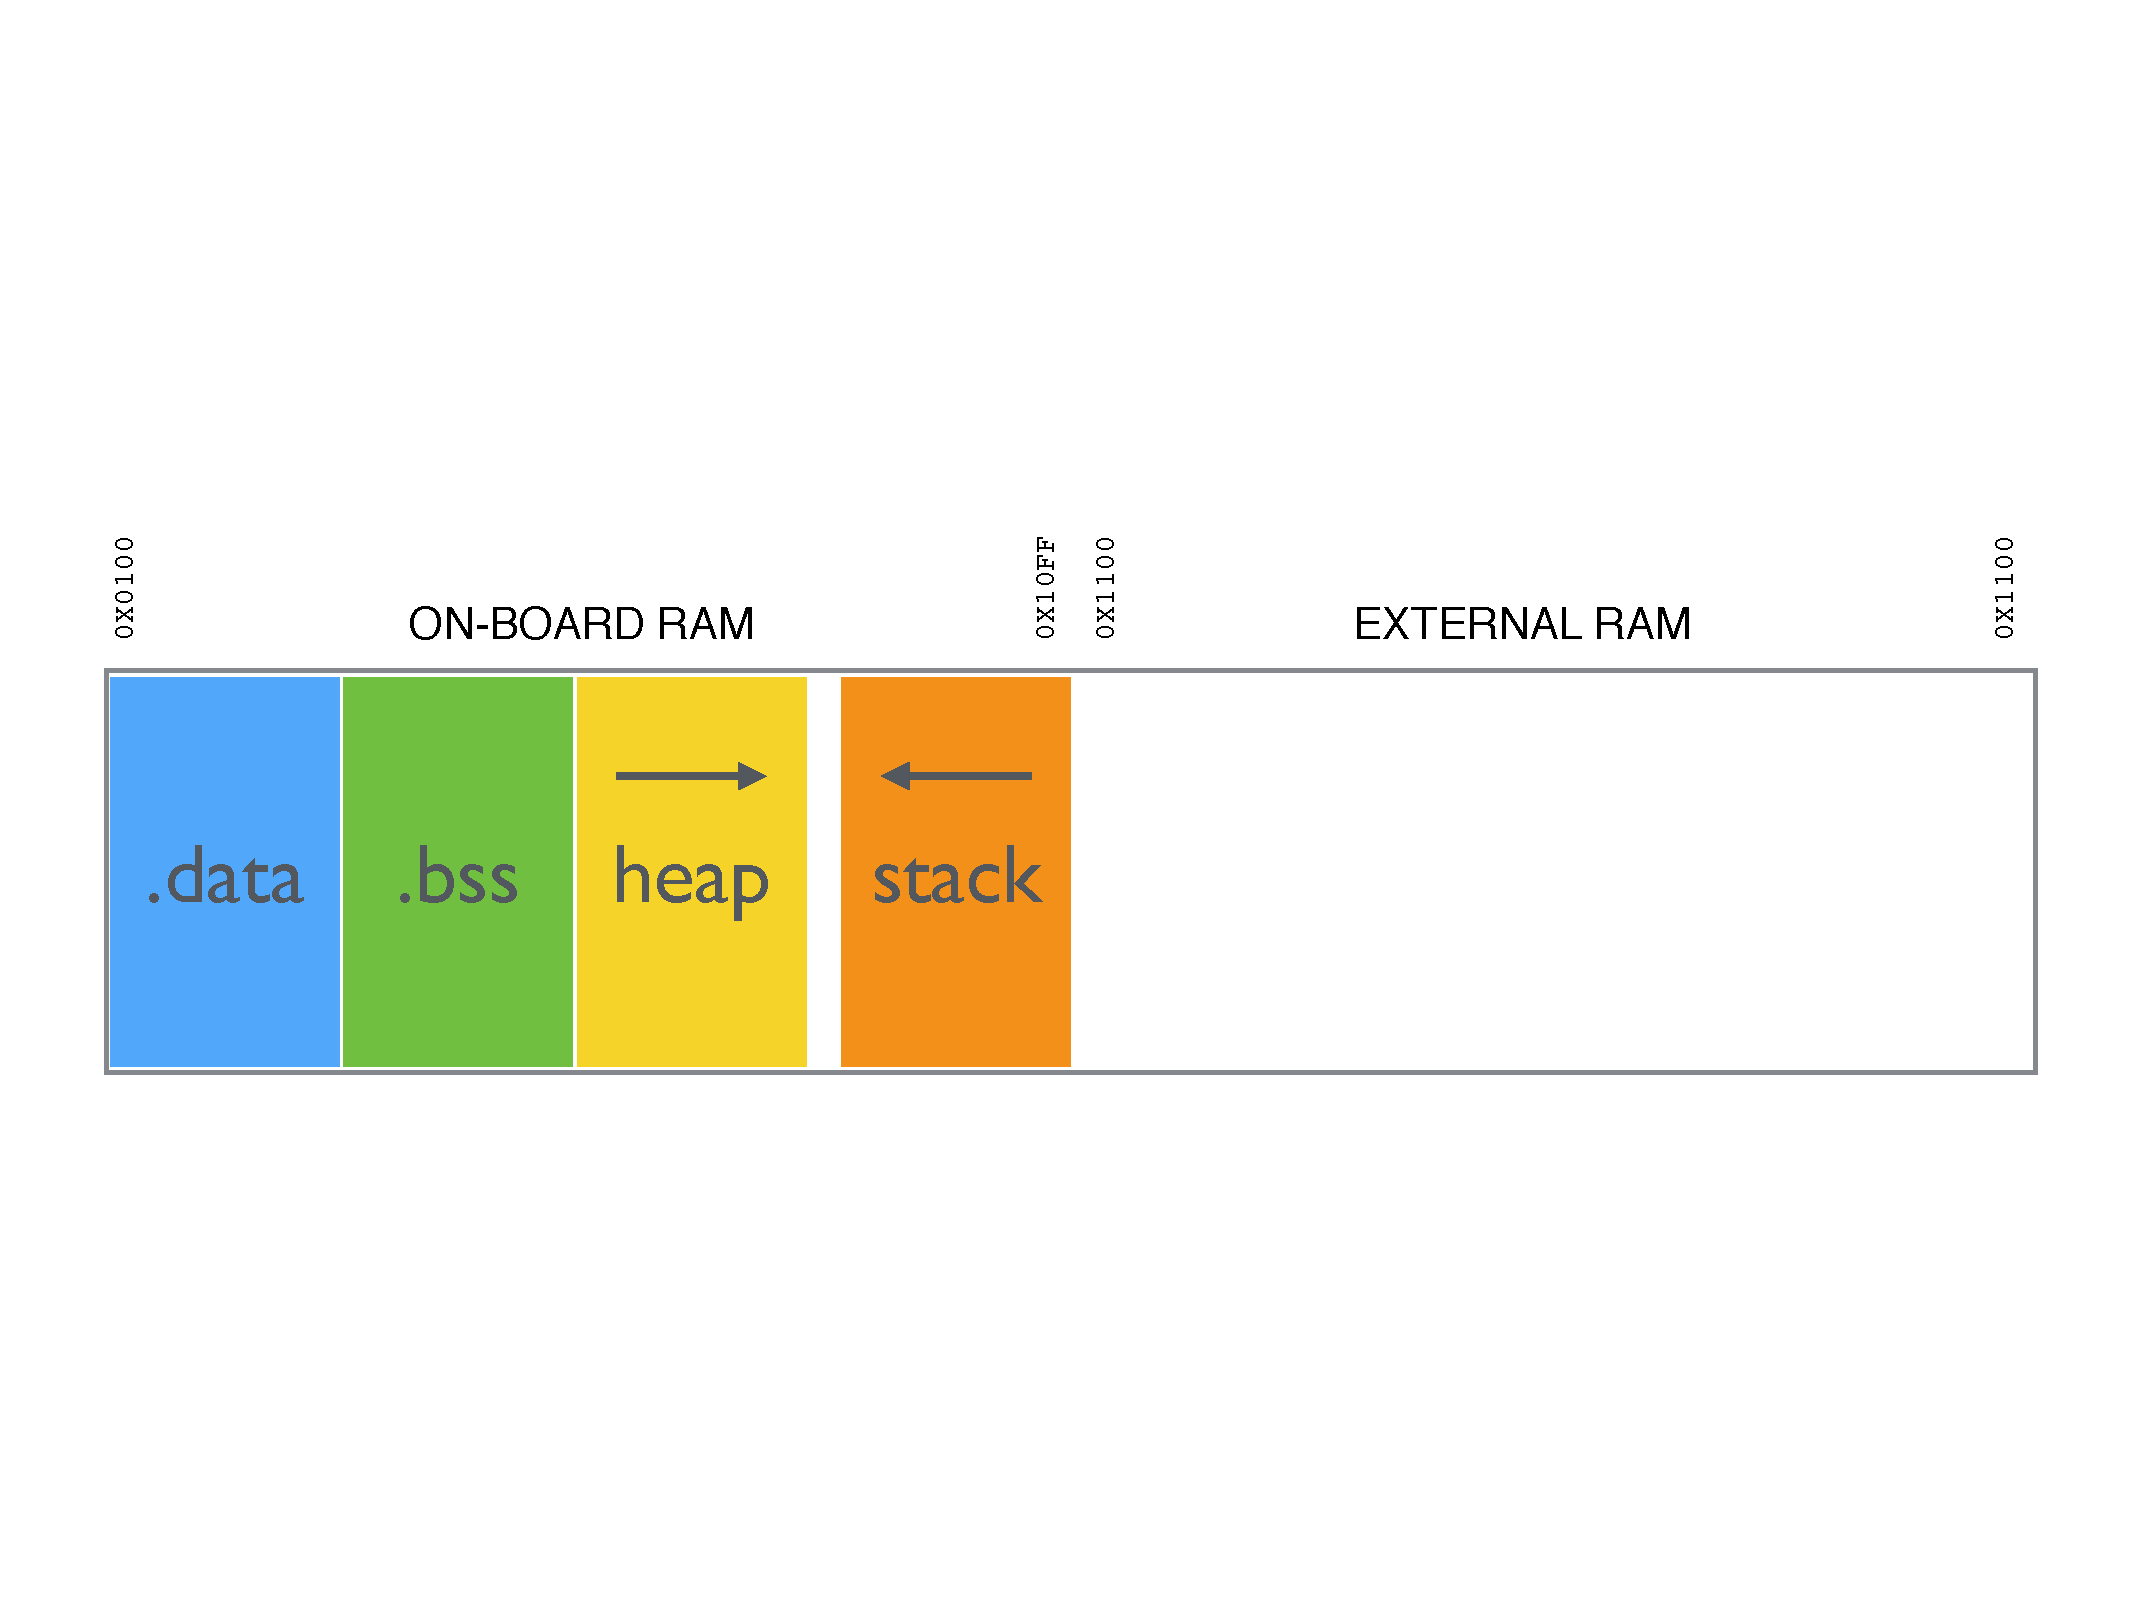
\includegraphics[width=2.5in]{resources/avr-ram-map.pdf}%
% \label{fig_first_case}}
% \hfil
% \subfloat[]{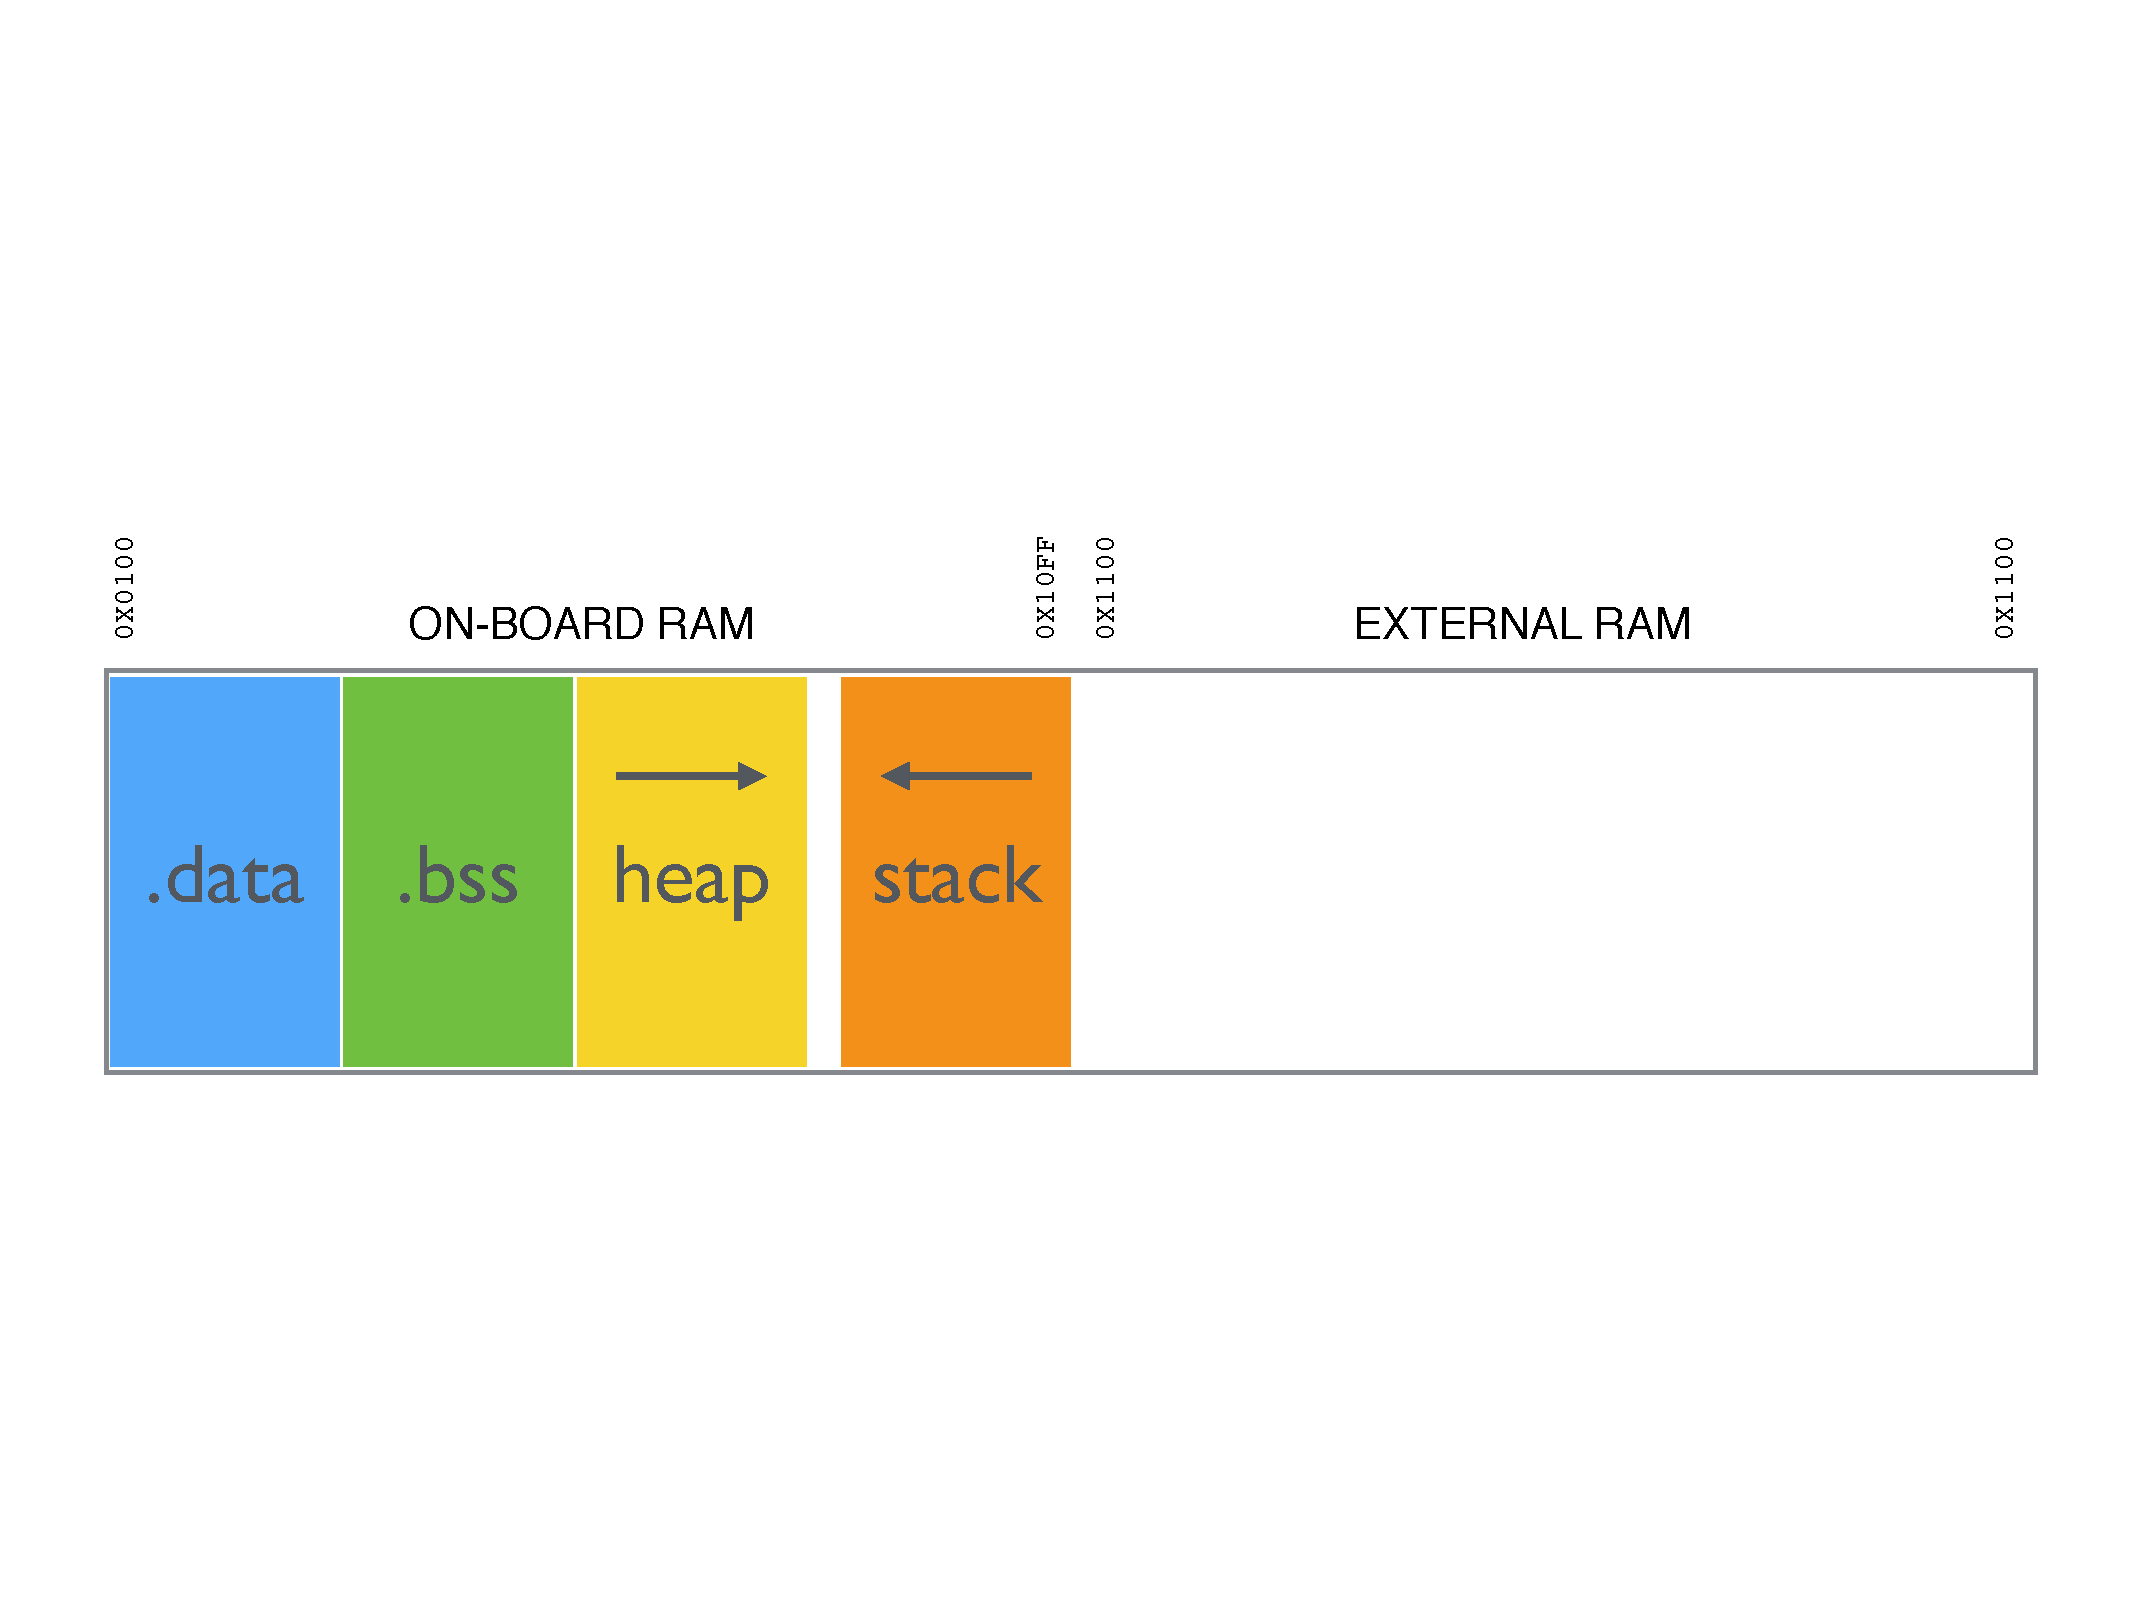
\includegraphics[width=2.5in]{resources/avr-ram-map.pdf}%
% \label{fig_second_case}}
% \caption{Simulation results: (a) Case I (b) Case II}
% \label{fig_sim2}
% \end{figure*}
% 
% \begin{table}[!t]
% \renewcommand{\arraystretch}{1.3}
% \caption{An Example of a Table}
% \label{table_example}
% \centering
% \begin{tabular}{|c||c|}
% \hline
% One & Two\\
% \hline
% Three & Four\\
% \hline
% \end{tabular}
% \end{table}


